\subsection*{Experimental setup}
In order to perform the experimental evaluation we used a tool to automatically
detect sentiment shift in tweets coming from year 2009 and regarding several
topics. We also downloaded news from the \emph{New York Times} and \emph{ABC
Australia} on the same topic and spanning on the same period of the tweets.

It's important to remember that tweet have different language structure that need to be normalized, so for cleaning purpose, the following operations were performed on the tweet text before starting the computation of all the different methodologies:
\begin{itemize}
	\item URLs removal from tweets using a regular expression
	\item conversion from Unicode to ASCII
\end{itemize}

In addition, while parsing the news, we considered the possibility that the
opinion expressed by tweets might be both delayed or in advance with respect to
news (e.g. if a movie becomes popular it is probable that news spread very fast
on twitter, but slower on newspaper, whereas other topics are discussed on
twitter only after news about them came out for several days). Thus, we
considered a enlarged time window for news which starts 5 days before the
beginning of the contradiction and last up to 5 days after the end of it.

After that, we manually labelled each contradiction point with the event which
caused it. 

The topics and contradiction points used for the experiments 
are showed in table \ref{tab:setup}. For each contradiction point we list its
symbolical name, the time interval in which it occurred, a description of the event
which we extracted by reading the tweet and a short label which synthesize it,
the number of news present in the contradiction interval $\pm 5$ days,
the correlation between news (all-to-all) and the correlation between news and tweets in the window.

To compute the \textbf{IntraNews} correlation: an algorithm calculate the NVS between all the possible couple created
using the news inside the time windows, then the IntraNews correlation is simple the average between the similarity value.
Likewise, the \textbf{News-Tweets} correlation is the NVS computed between tweet belonging to the contradiction points and 
news of the same time windows. The NVS is calculated between the contradiction tweet representation and the representation of all the news belonging to the same time windows. 

In detail the IntraNews correlation is a indicator of how much the news inside the time windows are similar one to the other,
instead the News-Tweets correlation indicate how much the news inside the time windows are correlate with the tweet.
Topic with high IntraNews correlation are easy to summarize since every news contains quite the same information,
on the other hand topic with high News-Tweets correlation are topic with low noise.
Both IntraNews and News-Tweets  correlations are calculated using N-gram tools.

\begin{table*}
	\centering
	\begin{tabularx}{\textwidth}{XX}
	
	\hline
\textbf{Contr. point:} Cern1 & \textbf{Contr. window:} 2009-10-29 - 2009-11-08\\
\multicolumn{2}{>{\setlength{\hsize}{2\hsize}\addtolength{\hsize}{2\tabcolsep}}X} {
	\textbf{Description:} On November 3rd a bird drops a
piece of bread which cause LHC overheating.
} \\
\textbf{Label:} bird accident & \textbf{Number of news in window $\pm 5$ days:} 3 \\
\textbf{IntraNews correlation:} 0.44437 & \textbf{News-Tweets correlation:} 0.3572 \\

	\hline
\textbf{Contr. point:} Cern2 & \textbf{Contr. window:} 2009-11-24 - 2009-12-04\\
\multicolumn{2}{>{\setlength{\hsize}{2\hsize}\addtolength{\hsize}{2\tabcolsep}}X} {
	\textbf{Description:} On November 30th LHC accelerates protons to an
energy of 1.18 TeV, becoming the world most powerful energy particle accelerator
} \\
\textbf{Label:} power on and record & \textbf{Number of news in window $\pm 5$ days:} 6 \\
\textbf{IntraNews correlation:} 0.25468 & \textbf{News-Tweets correlation:} 0.44832 \\

	\hline
\textbf{Contr. point:} FortHood & \textbf{Contr. window:} 2009-11-02 - 2009-11-06\\
\multicolumn{2}{>{\setlength{\hsize}{2\hsize}\addtolength{\hsize}{2\tabcolsep}}X} {
	\textbf{Description:} On November 5th a US marine kills 13 people
} \\
\textbf{Label:} shooting & \textbf{Number of news in window $\pm 5$ days:} 70 \\
\textbf{IntraNews correlation:} 0.26553 & \textbf{News-Tweets correlation:} 0.3582 \\

\hline
\textbf{Contr. point:} Hangover & \textbf{Contr. window:} 2009-06-21 - 2009-06-27\\
\multicolumn{2}{>{\setlength{\hsize}{2\hsize}\addtolength{\hsize}{2\tabcolsep}}X} {
	\textbf{Description:} People are entusiastic about the movie (released on June 5th)
} \\
\textbf{Label:} movie released & \textbf{Number of news in window $\pm 5$ days:} 5 \\
\textbf{IntraNews correlation:} 0.19866 & \textbf{News-Tweets correlation:} 0.37797 \\

\hline
\textbf{Contr. point:} Lcross & \textbf{Contr. window:} 2009-10-31 - 2009-11-08\\
\multicolumn{2}{>{\setlength{\hsize}{2\hsize}\addtolength{\hsize}{2\tabcolsep}}X} {
	\textbf{Description:} NASA publishes preliminary results on the Lcross missions.
	Other results are announced to be released in the next weeks
} \\
\textbf{Label:} preliminary findings & \textbf{Number of news in window $\pm 5$ days:} 0 \\
\textbf{IntraNews correlation:} 0 & \textbf{News-Tweets correlation:} 0 \\

\hline
\textbf{Contr. point:} Jackson1 & \textbf{Contr. window:} 2009-06-24 - 2009-06-27 \\
\multicolumn{2}{>{\setlength{\hsize}{2\hsize}\addtolength{\hsize}{2\tabcolsep}}X} {
\textbf{Description:} The singer dies on June 25th.}\\
\multicolumn{2}{>{\setlength{\hsize}{2\hsize}\addtolength{\hsize}{2\tabcolsep}}X} {
\textbf{Note:} This contradiction window was manually adjusted, since the automatically computed one is not centered on the main event.} \\
\textbf{Label:} Jackson's death & \textbf{Number of news in window $\pm 5$ days:} 143 \\
\textbf{IntraNews correlation:} 0.20704 & \textbf{News-Tweets correlation:} 0.26008 \\

\hline
\textbf{Contr. point:} Jackson2 & \textbf{Contr. window:} 2009-08-23 - 2009-08-29 \\
\multicolumn{2}{>{\setlength{\hsize}{2\hsize}\addtolength{\hsize}{2\tabcolsep}}X} {
	\textbf{Description:} On august 28th another popular
musician, Adam Goldstein, dies. The day after, August 29th is Jackson's
birthday
}\\
\textbf{Label:} Jackson birthday, Goldstein's death & \textbf{Number of news in window $\pm 5$ days:} 48 \\
\textbf{IntraNews correlation:} 0.23583 & \textbf{News-Tweets correlation:} 0.37050 \\

\hline
\textbf{Contr. point:} SwineFlu & \textbf{Contr. window:} 2009-06-19 - 2009-06-23 \\
\multicolumn{2}{>{\setlength{\hsize}{2\hsize}\addtolength{\hsize}{2\tabcolsep}}X} {
	\textbf{Description:} Swine flu is spreading around the world.
}\\
\textbf{Label:} pandemic & \textbf{Number of news in window $\pm 5$ days:} 31 \\
\textbf{IntraNews correlation:} 0.21648 & \textbf{News-Tweets correlation:} 0.20320 \\

\hline
	\end{tabularx}
	\caption{Contradiction points used for experimental evaluation}
	\label{tab:setup}
\end{table*}

Some interesting considerations can be drawn looking at the contradiction points.
First of all, you may notice, that, although our tool detected a \emph{sentiment
shift} in the \emph{Lcross} topic, no news can be found in the selected time period.
Similarly, the amount of news regarding other contradiction points is sometimes
very small; this is particularly true for scientific topics (e.g. \emph{Cern1},
\emph{Cern2}).
This fact will be further discussed at the end of this paper. Since there are no
news in the \emph{Lcross} contradiction point, we will omit it from following
experiments.

\subsection*{Experiments}
\subsubsection*{SpaceSaving evaluation}
Among all the possible SpaceSaving configuration, we chose to split news at
sentence level and to group them 2 by 2, since this seemed to be the best
configuration from some preliminary tests.

The results obtained by running it are showed in table \ref{tab:resultsSS}. For
each contradiction point the three best chunks are showed with their score, as well as the most
common words in the tweets (according to SpaceSaving) and their value.

As you may notice, some sentences are present more than once. This can be
justified either by repetition of the same sentence in the same news or by
articles citing previous ones.

\subsubsection*{Tf/idf evaluation}
In the table \ref{tab:resultsTfIdf} is possible to see the results of TF/IDF that is used as baseline and is possible compare other methods.

\subsubsection*{LSI evaluation}
LSI as for TF-IDF present a list of word for output that are reported on table \ref{tab:resultsLSI}. It's to mark down that the output, for FortHood topic, is cut due to paper readability motivations.



\subsubsection*{Ngram Graph evaluation}
In table \ref{tab:resultsNGG} are reported the obtained results with the correlation score of the best news. It's the maximum correlation value between a news and the contradiction tweet.
It's important to point out that, for presentation reasons, the summary reported is smaller respect the one created by the NGG methodologies and all the experiment reported where conduced with the default setting suggested by George Giannakopoulos of rank=3 and neighbourhood distance = 3

\subsubsection*{Description of the algorithm}
\emph{SpaceSaving} \cite{SS} is an algorithm which was first presented by Metwally et al.
in 2005 to efficiently compute the most frequent terms in a data stream. It
allows the user to find $k$ words which are among the most frequent in the given
stream. Although this is a heuristic algorithm whose result's correctness is not
guaranteed, SpaceSaving is able to specify the upper bound of the error for each
word presented as output.

The classic implementation is based on a fixed size list of tuple 
\begin{displaymath}
	(word, occurrencies, error)
\end{displaymath}
The stream is read word by word and at any time one of the following condition
is verified:
\begin{enumerate}
	\item \label{SS-among-frequent}
		the word is already in the list of frequent terms
	\item \label{SS-list-not-full}
		the word is not among the frequent terms, but the list is not full
	\item \label{SS-list-full}
		the word is not among the frequent terms and the list is full
\end{enumerate}
If the first condition is verified, then the algorithm will proceed incrementing
the number of occurrencies of that term; if condition \ref{SS-list-not-full} is
verified, instead, we add that word to the list of frequent terms with number of
occurrencies 1 and number of errors 0; if condition \ref{SS-list-full} is
verified, then we scan the list for the term with the lowest number of
occurrencies and replace it with the new word. When this replacement takes place
we set the number of errors equal to the number of occurrencies of the word we
just replaced, then we increment the number of occurrencies.

Our python implementation of this algorithm is slightly different from the
classic one described above, since we test the word against a list of stop words
and we added a hashmap to avoid useless
replacement. In our implementation, then, the following steps are performed:
\begin{enumerate}
	\item if the word is in the stop word lists, does nothing
	\item otherwise compute the hash of the given word
	\item increment the value associated to that hash
	\item check whether the value stored in the hash map is above the number of
		occurrencies of the less frequent term tracked by the SpaceSaving
		algorithm. If so, the replacement occurs, otherwise nothing happens.
\end{enumerate}
The output of this algorithm is a couple $(word, value)$ where the value is
computed as 
\begin{displaymath}
	value = occurrencies - error
\end{displaymath}
In order to reduce the noise we chose to use only couples where the value is
above a certain threshold.

\subsubsection*{Description of the methodology}
We have seen how we exploit the SpaceSaving algorithm to obtain the list of
frequent terms in a text and their
values. 

To accomplish our task, we ran the program described above on the set of tweets inside a
<<<<<<< HEAD
\emph{contradiction point}[CP], thus obtaining the list of frequent terms within the
contradiction; then, we read all the news which were published in the same time
period (a certain error between the publishing date and the contradiction
window) and for each of them we compute its score as
=======
\emph{contradiction pint} thus obtaining the list of frequent terms inside the
contradictions; then, we read all the news which were published during the
contradiction (a certain error between the publishing date and the contradiction
window might be taken in account) and for each of them we compute its score as
>>>>>>> 7a25539a6cb58d6ecc095f13a0f838184e4e830d
\begin{displaymath}
	newsScore = \sum_{w \in W} value(w)
\end{displaymath}
where $W$ is the list of words in the news and the value is null if that term is
not in the \emph{frequent term list}.

The news with the highest score is selected as the one causing the shift and its
first words are presented as output to the user.

This approach revealed to be very fast and from its formulation we can see that
it can be applied incrementally. As a drawback, we must say that it does not
take in account the background coming from the topic, hence it is not able to
discern whether a given frequent term is informative or not (e.g. running this
program on the Obama topic it is likely that the most
frequent terms will be ``President'', `Barack'', ``Obama'', ``USA'', hence a
news containing more repetitions of these words will have a high score, even if
those words are not informative at all)



\begin{table*}
	\centering
	\begin{tabularx}{\textwidth}{XXX}
\hline
\textbf{Contr. point:} Cern1 & \textbf{Label:} bird accident & \textbf{Number of news:} 3\\
\textbf{Jaccard similarity:} 0.052631\\
\multicolumn{3}{>{\setlength{\hsize}{3\hsize}\addtolength{\hsize}{3\tabcolsep}}X}
	{\textbf{Result:} "billion","minus","incident","degrees","bird","week","system","french","swiss","universe"} \\
\hline


\textbf{Contr. point:} Cern2 & \textbf{Label:} power on and record & \textbf{Number of news:} 6\\
\textbf{Jaccard similarity:} 0.17647\\
\multicolumn{3}{>{\setlength{\hsize}{3\hsize}\addtolength{\hsize}{3\tabcolsep}}X}
{\textbf{Result:}  "tev","lhc","teraelectronvolts","already","conditions","higgs","energy","dark","next","explain"} \\
\hline

\textbf{Contr. point:} Fort Hood & \textbf{Label:} shooting & \textbf{Number of news:} 56\\
\textbf{Jaccard similarity:} 0.17647\\ 
\multicolumn{3}{>{\setlength{\hsize}{3\hsize}\addtolength{\hsize}{3\tabcolsep}}X}
{\textbf{Result:} "update", "base", "reports", "killed", "gunman", "hasan", "wounded", "soldiers", "hood", "fort"
} \\
\hline


\textbf{Contr. point:} Hangover & \textbf{Label:} movie released & \textbf{Number of news:} 5\\
\textbf{Jaccard similarity:} 0.052631\\ 
\multicolumn{3}{>{\setlength{\hsize}{3\hsize}\addtolength{\hsize}{3\tabcolsep}}X}
{\textbf{Result:} "cbs", "election", "hybrid", "moussavi", "ahmadinejad", "bermuda", "it's", "iranian", "vote", "going"  
} \\
\hline


\textbf{Contr. point:} Lcross & \textbf{Label:} preliminary findings & \textbf{Number of news:} 0\\
\textbf{Jaccard similarity:} 0\\ 
\multicolumn{3}{>{\setlength{\hsize}{3\hsize}\addtolength{\hsize}{3\tabcolsep}}X}
{\textbf{Result:} \emph{No news in the selected time period}} \\
\hline


\textbf{Contr. point:} Jackson1 & \textbf{Label:} Jackson's death & \textbf{Number of news:} 83\\
\textbf{Jaccard similarity:} 0.16667\\ 
\multicolumn{3}{>{\setlength{\hsize}{3\hsize}\addtolength{\hsize}{3\tabcolsep}}X}
{\textbf{Result:} "playing", "jackson\u2019s", "michael", "jackson"}  \\
\hline


\textbf{Contr. point:} Jackson2 & \textbf{Label:} Jackson birthday, Goldstein's death & \textbf{Number of news:} 47\\
\textbf{Jaccard similarity:} 0.17647\\
\multicolumn{3}{>{\setlength{\hsize}{3\hsize}\addtolength{\hsize}{3\tabcolsep}}X}
{\textbf{Result:} "theater", "apollo", "jackson's", "fame", "memorial", "place", "fans", "take", "death", "jackson"
}  \\
\hline

\textbf{Contr. point:} SwineFlu & \textbf{Label:} pandemic & \textbf{Number of news:} 28\\
\textbf{Jaccard similarity:}0.133333\\
\multicolumn{3}{>{\setlength{\hsize}{3\hsize}\addtolength{\hsize}{3\tabcolsep}}X}
{\textbf{Result:} "deaths", "conditions", "confirmed", "number", "department", "swine", "flu"} \\
\hline


\textbf{Contr. point:} Lcross & \textbf{Label:} preliminary findings & \textbf{Number of news:} 0\\
\textbf{Jaccard similarity:} 0\\ 
\multicolumn{3}{>{\setlength{\hsize}{3\hsize}\addtolength{\hsize}{3\tabcolsep}}X}
{\textbf{Result:} \emph{No news in the selected time period}} \\
\hline


\textbf{Contr. point:} Jackson1 & \textbf{Label:} Jackson's death & \textbf{Number of news:} 83\\
\textbf{Jaccard similarity:} 0.166667\\ 
\multicolumn{3}{>{\setlength{\hsize}{3\hsize}\addtolength{\hsize}{3\tabcolsep}}X}
{\textbf{Result:} "playing", "jackson\u2019s", "michael", "jackson"}  \\
\hline


\textbf{Contr. point:} Jackson2 & \textbf{Label:} Jackson birthday, Goldstein's death & \textbf{Number of news:} 47\\
\textbf{Jaccard similarity:} 0.17647\\
\multicolumn{3}{>{\setlength{\hsize}{3\hsize}\addtolength{\hsize}{3\tabcolsep}}X}
{\textbf{Result:} "theater", "apollo", "jackson's", "fame", "memorial", "place", "fans", "take", "death", "jackson"
}  \\
\hline

\textbf{Contr. point:} SwineFlu & \textbf{Label:} pandemic & \textbf{Number of news:} 28\\
\textbf{Jaccard similarity:}0.133333\\
\multicolumn{3}{>{\setlength{\hsize}{3\hsize}\addtolength{\hsize}{3\tabcolsep}}X}
{\textbf{Result:} "deaths", "conditions", "confirmed", "number", "department", "swine", "flu"} \\
\hline


	\end{tabularx}
	\caption{Results achieved using Tf-Idf}
	\label{tab:resultsTfIdf}
\end{table*}



\begin{table*}
	\centering
	\begin{tabularx}{\textwidth}{XXX}
\hline
\textbf{Contr. point:} Cern1 & \textbf{Label:} bird accident & \textbf{Number of news:} 3\\
\textbf{LSI similarity:} 0.38780\\
\multicolumn{3}{>{\setlength{\hsize}{3\hsize}\addtolength{\hsize}{3\tabcolsep}}X}
	{\textbf{Result:} "billion","week","collider","cern","universe","system","french","bird","incident","degrees","swiss","last","minus"} \\
\hline


\textbf{Contr. point:} Cern2 & \textbf{Label:} power on and record & \textbf{Number of news:} 6\\
\textbf{LSI similarity:} 0.76391\\
\multicolumn{3}{>{\setlength{\hsize}{3\hsize}\addtolength{\hsize}{3\tabcolsep}}X}
{\textbf{Result:}  "teraelectronvolts", "already", "accelerator", "energy", "year", "tev", "collider", "explain", "next", "scientists", "new", "conditions", "big", "dark", "bang", "billion", "lhc", "particle","higgs", "cern", "swiss", "physics"} \\
\hline

\textbf{Contr. point:} Fort Hood & \textbf{Label:} shooting & \textbf{Number of news:} 70\\
\textbf{LSI similarity:} 0.63983\\ 
\multicolumn{3}{>{\setlength{\hsize}{3\hsize}\addtolength{\hsize}{3\tabcolsep}}X}
{\textbf{Result:} "luby's", "nadal", "shot", "being", "over", "soon", "rest", "sources", "wounded", "scott", "haug", "go", "soldiers",\ldots
} \\
\hline


\textbf{Contr. point:} Hangover & \textbf{Label:} movie released & \textbf{Number of news:} 5\\
\textbf{LSI similarity:} 0.13677\\ 
\multicolumn{3}{>{\setlength{\hsize}{3\hsize}\addtolength{\hsize}{3\tabcolsep}}X}
{\textbf{Result:} "right", "tough", "people", "hybrid", "yeah", "one", "cbs", "see", "through", "moussavi", "vote", "rally", "yes", "ahmadinejad", "little", "it's", "percent", "actually", "going", "gets", "more", "iran", "first", "yesterday", "here", "news", "now", "those", "they're", "here's", "iranian", "car", "well", "bermuda", "thing", "wins", "mean", "think", "election"
} \\
\hline


%\textbf{Contr. point:} Lcross & \textbf{Label:} preliminary findings & \textbf{Number of news:} 0\\
%\textbf{LSI similarity:} 0\\ 
%\multicolumn{3}{>{\setlength{\hsize}{3\hsize}\addtolength{\hsize}{3\tabcolsep}}X}
%{\textbf{Result:} \emph{No news in the selected time period}} \\
%\hline


\textbf{Contr. point:} Jackson1 & \textbf{Label:} Jackson's death & \textbf{Number of news:} 95\\
\textbf{LSI similarity:} 0.84014\\
\multicolumn{3}{>{\setlength{\hsize}{3\hsize}\addtolength{\hsize}{3\tabcolsep}}X}
{\textbf{Result:} "jackson", "jackson's", "michael", "playing"
}  \\
\hline


\textbf{Contr. point:} Jackson2 & \textbf{Label:} Jackson birthday, Goldstein's death & \textbf{Number of news:} 48\\
\textbf{LSI similarity:} 0.62625\\ 
\multicolumn{3}{>{\setlength{\hsize}{3\hsize}\addtolength{\hsize}{3\tabcolsep}}X}
{\textbf{Result:} "clip", "show", "series", "tuesday", "one", "gomes", "reunion", , "special", "before", "jackson", "family", "tito", "reporter", "few", "randy", "details", "lot", "weeks", "footage", "jermaine", "brothers", "intimate", "described", "hour", "marlon", "jackson's", "months", "michael", "jackie"}  \\

\hline

\textbf{Contr. point:} SwineFlu & \textbf{Label:} pandemic & \textbf{Number of news:} 31\\
\textbf{LSI similarity:} 0.72671\\
\multicolumn{3}{>{\setlength{\hsize}{3\hsize}\addtolength{\hsize}{3\tabcolsep}}X}
{\textbf{Result:} "control", "bell", "doing", "schools", "officials", "rooms", "ga", "home", "hospitals", "children", "staff", "hospital", "thursday", "symptoms", "enough", "parents", "sick", "week", "masks", "tested", "protection", "members", "front", "cases", "dr", "care", "reported", "camp", "flu", "identified", "patients", "swine", "camps"} \\
\hline



	\end{tabularx}
	\caption{Results achieved using LSI}
	\label{tab:resultsLSI}
\end{table*}



\begin{table*}
	\centering
	\begin{tabularx}{\textwidth}{XXXX}
\hline
\textbf{Contr. point:} Cern1 & \textbf{Label:} bird accident & \textbf{Number of news:} 3\\
\textbf{Summary mean:} 0.35988 & \textbf{Best news:} 0.37512 & \textbf{News homogeneity:} 0.44437 & \textbf{News-Tweet avg:} 0.3582\\
\multicolumn{4}{>{\setlength{\hsize}{4\hsize}\addtolength{\hsize}{4\tabcolsep}}X}
	{\textbf{Result:} bird escaped unharmed but lost its bread,' CERN said in a statement. The 27 kilometre-long particle collider, which runs in a circular tunnel under the French-Swiss border near Geneva, has been plagued by problems since it was briefly started in September 2008. CERN said the latest incident was minor and did not affect attempts to restart the accelerator later this month following repairs.
	
	It was the first time protons have traveled in the giant particle accelerator since last September when the first attempts to turn on the \$6 billion machine ended in a fury of sparks and smoke \ldots
} \\
\hline


\textbf{Contr. point:} Cern2 & \textbf{Label:} power on and record & \textbf{Number of news:} 6\\
\textbf{Summary mean:} 0.4856 &\textbf{Best news:} 0.50583 & \textbf{News homogeneity:} 0.25468 & \textbf{News-Tweet avg:} 0.44832 \\
\multicolumn{4}{>{\setlength{\hsize}{4\hsize}\addtolength{\hsize}{4\tabcolsep}}X}
{\textbf{Result:}  The European Organisation for Nuclear Research (CERN) says two beams of protons circulating simultaneously led to collisions at least four times during the afternoon and evening.


CERN’s director, Rolf Heuer, said in a statement, “It’s great to see beam circulating in the LHC again,” but he and others cautioned that there was a long way to go before the collider started producing the physics it was designed for\ldots
} \\
\hline

\textbf{Contr. point:} Fort Hood & \textbf{Label:} shooting & \textbf{Number of news:} 70\\
\textbf{Summary mean:} 0.4855 &\textbf{Best news:} 0.50583 & \textbf{News homogeneity:} 0.26553  & \textbf{News-Tweet avg:} 0.3582\\ 
\multicolumn{4}{>{\setlength{\hsize}{4\hsize}\addtolength{\hsize}{4\tabcolsep}}X}
{\textbf{Result:} This signals that the killings at Fort Hood are seen less as part of the ongoing conflict between America and the Muslim world, or the wars in Iraq and Afghanistan, and more as part of a larger context of violent crime in the United States.


But the investigators, working with behavioral experts, suggested that he might have long suffered from emotional problems that were exacerbated by the tensions of his work with veterans of the wars in Iraq and Afghanistan who returned home with serious psychiatric problems
\ldots
} \\
\hline

\textbf{Contr. point:} Hangover & \textbf{Label:} movie released & \textbf{Number of news:} 5\\
\textbf{Summary mean:} 0.41346 & \textbf{Best news:} 0.41346 & \textbf{News homogeneity:} 0.19866 & \textbf{News-Tweet avg:} 0.37797\\
\multicolumn{4}{>{\setlength{\hsize}{4\hsize}\addtolength{\hsize}{4\tabcolsep}}X}
{\textbf{Result:} In my conversations with people in the movie business, it was clear that they were caught completely off guard, and many are livid at the prospect of a diminishing of what has been the most hallowed award in all of entertainment (and that somehow, the academy board, drawn from the most gossip-riddled industry in the land, managed to keep a secret until it was a fait accompli).
Executives argue that the best-picture award continues to have resonance with consumers when used as a laurel in ads precisely because it is such a rare jewel, and that the Oscars have maintained their distance from secondary awards like the Golden Globes and the Broadcast Film Critics Association by nominating five best, not 10.
\ldots
} \\
\hline


\textbf{Contr. point:} Lcross & \textbf{Label:} preliminary findings & \textbf{Number of news:} 0\\
\textbf{Summary mean:} 0 & \textbf{Best news:} 0 & \textbf{News homogeneity:} 0 & \textbf{News-Tweet avg:} 0\\
\multicolumn{4}{>{\setlength{\hsize}{4\hsize}\addtolength{\hsize}{4\tabcolsep}}X}
{\textbf{Result:} \emph{No news in the selected time period}} \\
\hline


\textbf{Contr. point:} Jackson1 & \textbf{Label:} Jackson's death & \textbf{Number of news:} 95\\
\textbf{Summary mean:} 0.63124 & \textbf{Best news:} 0.64663 & \textbf{News homogeneity:} 0.23583 & \textbf{News-Tweet avg:} 0.54462\\
\multicolumn{4}{>{\setlength{\hsize}{4\hsize}\addtolength{\hsize}{4\tabcolsep}}X}
{\textbf{Result:} "Court documents suggest that the drug was administered by a doctor at Mr. Jackson’s request.


According to court documents that were unsealed on Monday, Dr. Conrad Murray, who was treating Mr. Jackson for insomnia, told investigators that he 


gave the singer propofol on that day after administering other drugs, including valium, lorazepam and midazolam.
\ldots
}  \\
\hline


\textbf{Contr. point:} Jackson2 & \textbf{Label:} Jackson birthday, Goldstein's death & \textbf{Number of news:} 48\\
\textbf{Summary mean:} 0.30598  & \textbf{Best news:} 0.31770 & \textbf{News homogeneity:} 0.21324 & \textbf{News-Tweet avg:} 0.22579\\
\multicolumn{4}{>{\setlength{\hsize}{4\hsize}\addtolength{\hsize}{4\tabcolsep}}X}
{\textbf{Result:} “Video | A reprise of a popular clip, given the Michael Jackson news:

It’s the Michael Jackson music channel.

“Backstage, Riccardo Tisci said the Givenchy show paid homage to Michael Jackson, as he was working on the costumes for his tour.”
\ldots
}  \\
\hline

\textbf{Contr. point:} SwineFlu & \textbf{Label:} pandemic & \textbf{Number of news:} 31\\
\textbf{Summary mean:} 0.27143  & \textbf{Best news:} 0.28586 & \textbf{News homogeneity:} 0.21648 & \textbf{News-Tweet avg:} 0.20320\\
\multicolumn{4}{>{\setlength{\hsize}{4\hsize}\addtolength{\hsize}{4\tabcolsep}}X}
{\textbf{Result:} The Israeli president, Shimon Peres, was tested and found to be clear of swine flu after he met with a group of 120 American young adults on an educational program and Israeli soldiers, many of whom turned out to be infected with the virus, a spokeswoman said Wednesday.


Updated, 11:58 p.m. |  Seven more deaths of people with swine flu have been confirmed, raising the number of deaths linked with the outbreak to 30, the New York City Department of Health and Mental Hygiene reported on Friday afternoon.
\ldots} \\
\hline

	\end{tabularx}
	\caption{Results achieved using N-gram graph}
	\label{tab:resultsNGG}
\end{table*}



\subsubsection*{NGG performance}
All the experiment about Ngram graph where conduced on a 2,4 GHz Intel Core 2 Duo with 4 GB 1067 MHz DDR3 RAM memory.
 All the code was compiled with intellij IDEA on Java 1.8 language. 
The reported test where conduced on Cern topic data set, since is the one that have multiple contradiction points and allowed us to test the methodology changing the following parameter:
\begin{itemize}
	\item rank of the graph
	\item neighbourhood distance[ND]
	\item time windows
\end{itemize}


In figure \ref{fig:et-fixed-10days-r-rank} is reported the computational time respect the neighbourhood distance for different rank values. 
It is easy to notice how for all the rank there is an exponential behaviour respect to the neighbourhood distance. 
Enlarging ND cause an exponential increasing of the edges number that a graph contains, so the computation time became exponentially longer.

\begin{figure*}[htbp]
	\centering
			{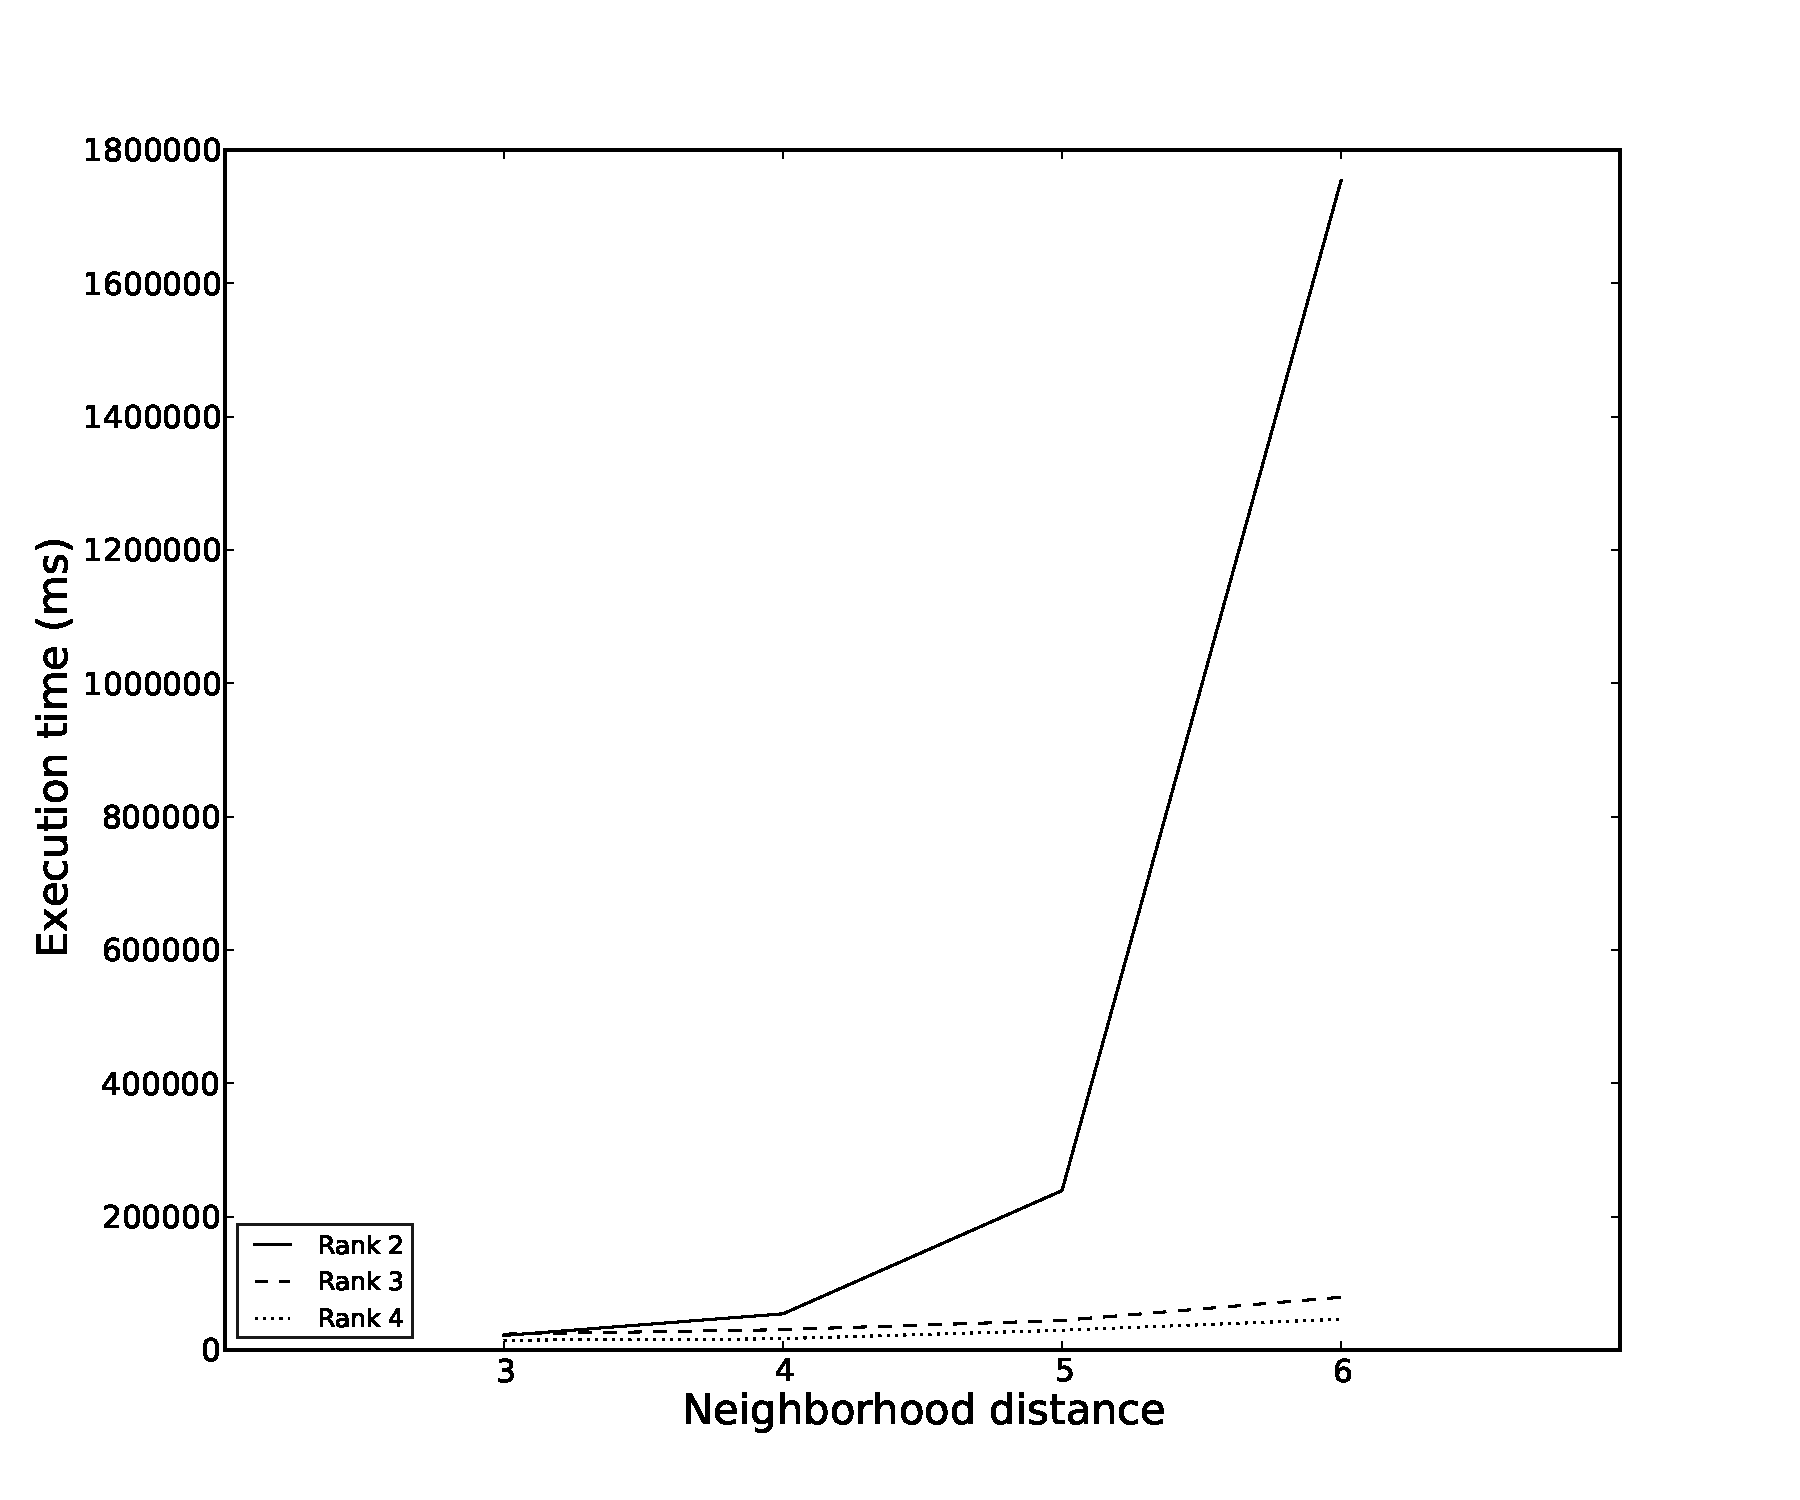
\includegraphics[width=5cm,height=5cm]{image/win_2_ranks.pdf}}	
		\caption[et-fixed-10days-r-rank]{Execution time for different rank value}
	\label{fig:et-fixed-10days-r-rank}
\end{figure*} 

In figure \ref{fig:et-fixed-10days-r-nd} is possible to see how the computation time change respect to the rank value at different neighbourhood distance. 
It's possible to see how if we increasing the rank, the computational time is quite the same. Seems that rank can mitigate the neighbourhood distance effect. 

The computation time for of the 2-gram diverge, instead 3-gram became more similar at the 4-gram behaviour. Probably because computing the similarity between 2-gram graph is an operation quite expensive since they have many edges to check.
Indeed neighbourhood distance is a less impactive parameter, 3 o 4 have quite the same computational time.

\begin{figure*}[htbp]
	\centering
			{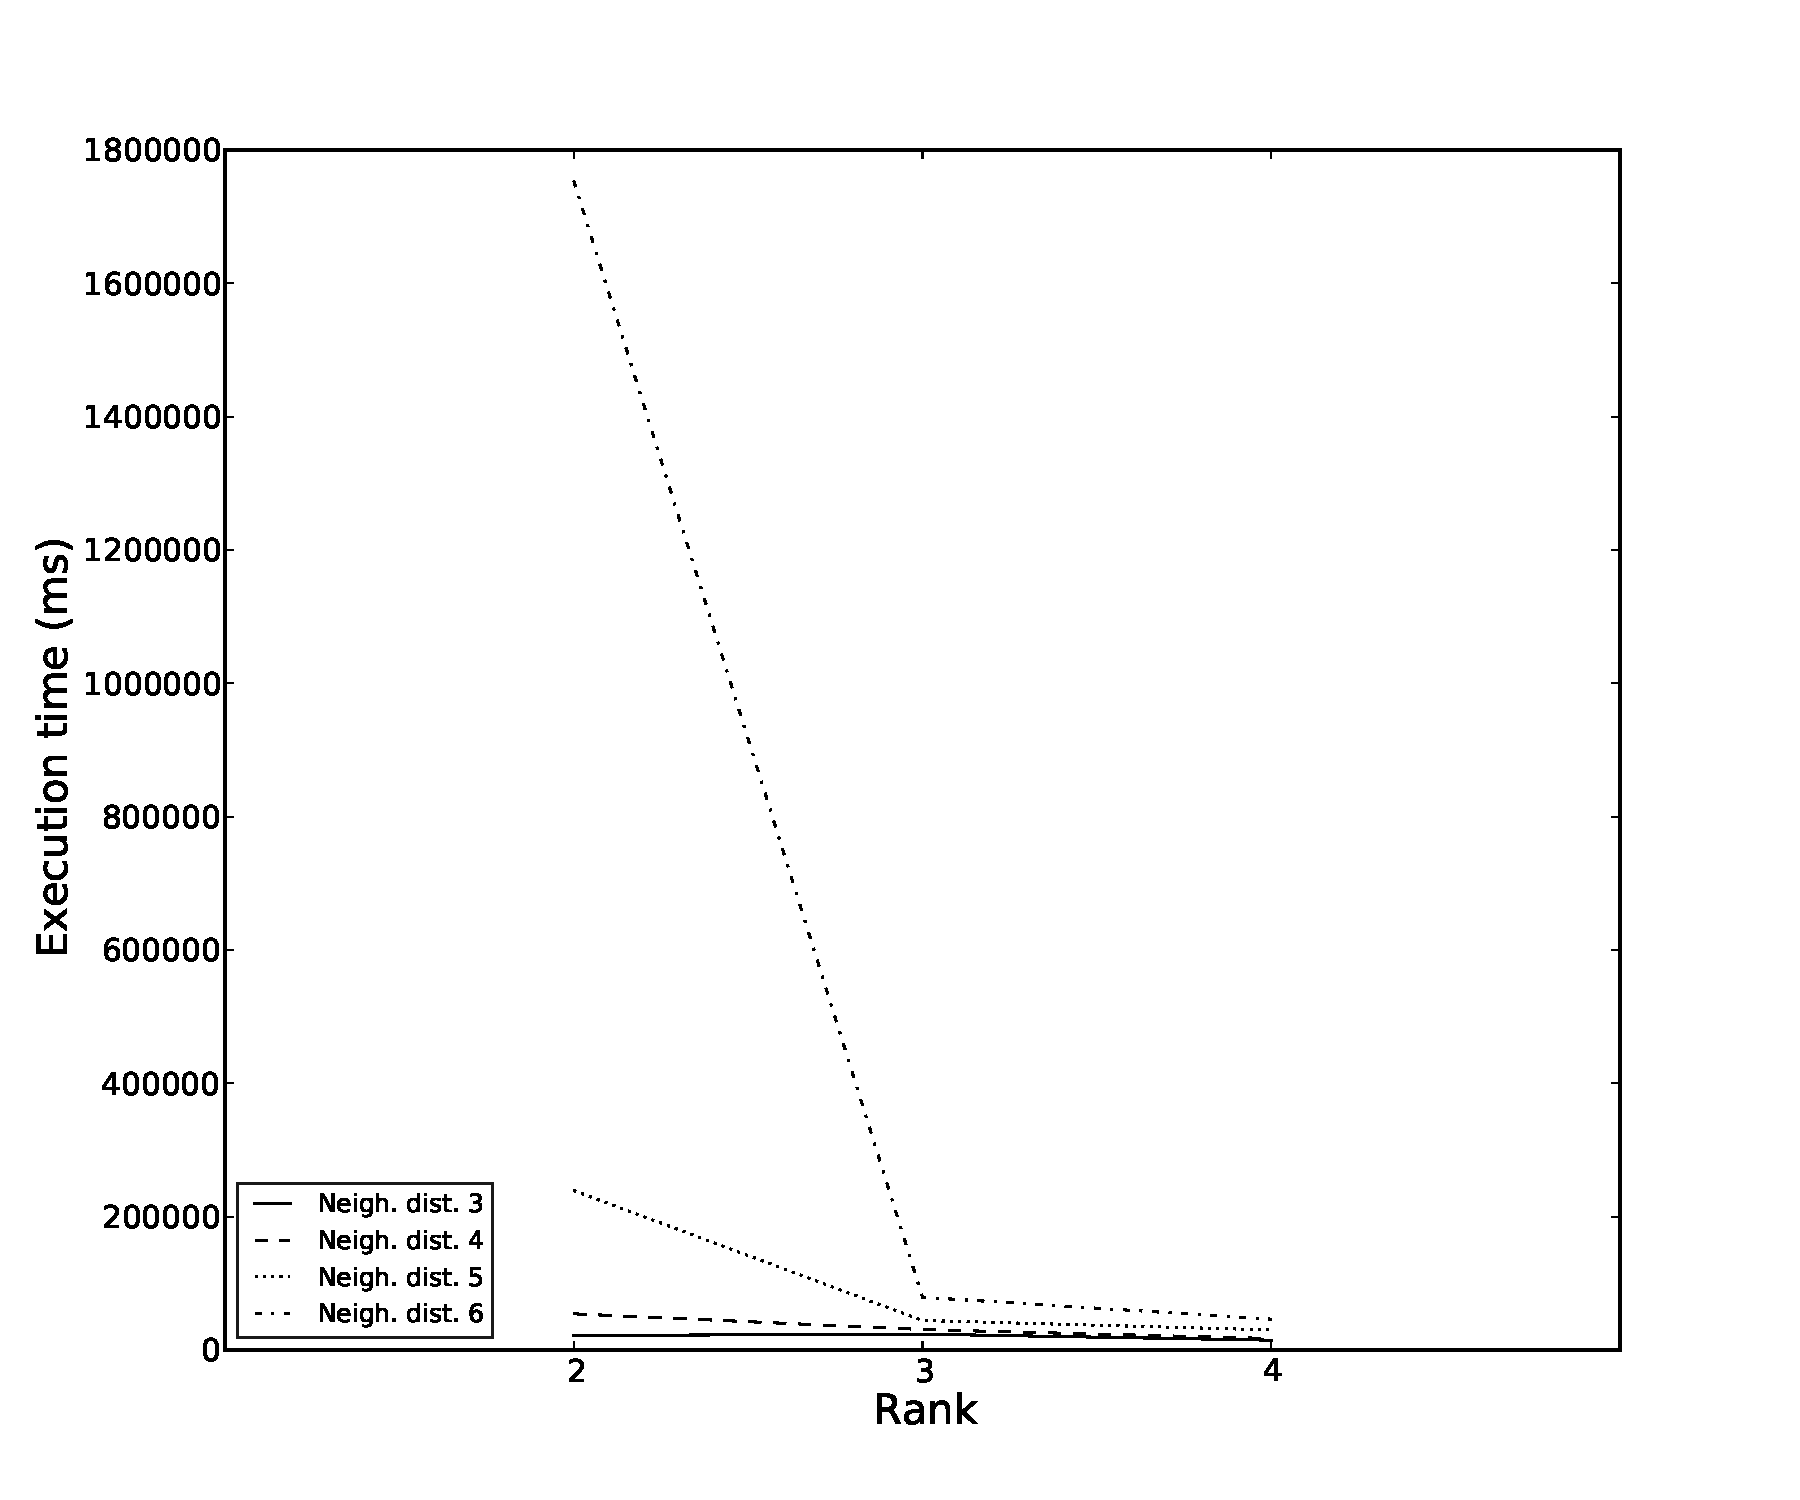
\includegraphics[width=5cm,height=5cm]{image/win_2_ndists.pdf}}	
	\label{fig:et-fixed-10days-r-nd}
\end{figure*} 

For what concern the summary point of view the neighbourhood distance factor has little influence on the summary since changing his value just produce a swapping on the order of the sentence in the summary.
In particular for a rank = 3 we obtain the following summary:
\begin{enumerate}
	\item CERN said the latest incident was minor and did not affect attempts to restart the accelerator later this month following repairs.
	\item 'The bird escaped unharmed but lost its bread,'CERN said in a statement.
	\item Bits of a French loaf dropped on an external electrical power supply caused a short circuit last week, triggering failsafe devices that shut down part of the cooling system of the giant experiment to probe the secrets of the universe.
	\item The bird was believed to be an owl.
	\item The European Organisation for Nuclear Research (CERN) says the system was restored several hours after the incident last week while the multi-billion-dollar Large Hadron Collider was barely affected.
	\item The 27 kilometre-long particle collider, which runs in a circular tunnel under the French-Swiss border near Geneva, has been plagued by problems since it was briefly started in September 2008.
\end{enumerate}

instead for a rank = 6 we obtain the summary
\begin{enumerate}
	\item CERN said the latest incident was minor and did not affect attempts to restart the accelerator later this month following repairs.
	\item Bits of a French loaf dropped on an external electrical power supply caused a short circuit last week, triggering failsafe devices that shut down part of the cooling system of the giant experiment to probe the secrets of the universe.
	\item The European Organisation for Nuclear Research (CERN) says the system was restored several hours after the incident last week while the multi-billion-dollar Large Hadron Collider was barely affected.
	\item 'The bird escaped unharmed but lost its bread,'CERN said in a statement. 
	\item The bird was believed to be an owl.
	\item The 27 kilometre-long particle collider, which runs in a circular tunnel under the French-Swiss border near Geneva, has been plagued by problems since it was briefly started in September 2008.
\end{enumerate}

This means that the rank has just a little effect of the order of the sentence, but not on the news-tweet correlation.
Knowing that neighbourhood distance strongly affect the computational time and slightly change the summary; it is reasonable to use a ND between 3 and 4 as suggested by the N-gram graph creator


%Figure \ref{fig:et-fixed-r3-winds} report the variation of computation time for fixed rank value(3). The shape of the computation time in this case is always the same: exponential respect the ND. 
%Notice that the max computation time always increase with the increasing of the windows size, since the algorithm have to compute the similarity between more news. In this way we can derive that the number of news, inside the time windows, affect the computation time in a almost linear way.


